% \begin{preamble}
\documentclass[12pt]{article}
\usepackage[margin=1in]{geometry}
\usepackage[utf8]{inputenc}
\renewcommand{\rmdefault}{phv} % Arial Font
\renewcommand{\sfdefault}{phv} % Arial Font
\usepackage{color}
\usepackage{tcolorbox}
\usepackage{graphicx}
\usepackage{ragged2e}
\graphicspath{ {./figures/}} % Location of the graphics files
\usepackage[labelfont=bf]{caption}
\usepackage{multicol}
\usepackage{nopageno} % remove page numbers
\pagestyle{empty} % remove page numbers
\usepackage{gb4e}
\noautomath
% \end{preamble}

\newcommand{\glr}{\textcolor{teal}}
\definecolor{Purple}{RGB}{255,10,140}
\newcommand{\jd}[1]{\textcolor{Purple}{[jd: #1]}}
\newcommand{\mm}[1]{\textcolor{teal}{[mm: #1]}}


\begin{document}
% Title
\centerline{\textbf{Affect First? Evaluating the Affect First Hypothesis Through Valence}}
% \centerline{Morgan Moyer, Anouch Bourmayan (Sorbonne University), Isidora Stojanovic and Brent Strickland (Jean-Nicod, ENS-PSL/CNRS}
% \centerline{mcmoyer11@gmail.com}%names
% Endtitle 
\centerline{We would like to be considered for the special session on valence.}
\normalsize
\bigskip

\noindent \textbf{Introduction}
If someone on the street yelled, ``Hey f*ck you!'', you would feel quite flummoxed and not a little emotional. For expletive expressions, the negative valence is a core component of their meaning. Words also have a dimension of meaning that can be described as Conceptual: the verb `love' is generally considered as having a positive valence, but also generally describes a psychological/abstract event or state of being. In contrast, `hug', while also of positive valence, more describes a physical/concrete event or state of being. The \textbf{Affect First Hypothesis} (AFH) is the psychological hypothesis that affective information is processed before conceptual information [1,2]. In the domain of word meaning and the lexicon, it would predict that affective meaning is accessed prior to conceptual meaning. Concretely, that judgments of a word's valence should be made faster than judgements of a word's conceptual feature(s). This appears true for expletives and slurs, whose affective meaning often triggers a concomitant physiological response (``hot'' affect). Does it hold for `love'/`hug' where judging them positive probably doesn't entail an elevated heart rate or sweaty palms (``cold'' affect)? We present several experiments that provide some evidence in support of the AFH. We ask two questions:

% If a long thin projectile is hurled at you, your instict likely is to duck, potentially in fear. 
% You probably felt your heart rate accelerate, your palms sweaty, and the sharp release of adrenaline that compelled you to action. 
% This emotion-first response occurs before you identify what the unidentified flying object is. 

% \vspace{-.3cm}
\begin{tcolorbox}[colback=white]
% \vspace{-.2cm}
\centering
\textbf{Q1 (specific)}: Are valence judgments cognitively prior to conceptual judgments? \\ 
\textbf{Q2 (broad)}: How should word valence be represented in the lexicon?
% \vspace{-.2cm}
\end{tcolorbox}
% \vspace{-.2cm}

\noindent \textbf{Background}
The last 20 years have seen a rise in the study of not-strictly-truth-conditional aspects of meaning which had previously been sidelined from semantic analysis in Fregean traditions. Affective meaning forms a natural class with slurs, expressivity, and evaluativity [3-9]. In XPrag studies on slur processing, the affective component of meaning has been found to aid the hearer in anticipating the speaker's referential intentions [10]. Neuroscientific research has shown mixed evidence for AFH, or ``affect effects'' [11-15], but recent research has emphasized the role that contextual information--writ large--plays in the modulation of affect effects, for example Task effects [15,16] and the communicative situation [17a]. One challenge to testing AFH is finding a conceptual dimension that makes a good comparison for affective judgments, because words can vary greatly on which conceptual dimension(s) best track(s) their meaning [18a-21]. We pit Valence against multiple conceptual categories to answer Q1/Q2. We present pilot data that seem to support AFH and the central role of valence for word meaning.\\


\noindent \textbf{Experiments 1 and 2: Categorization tasks (Q1)}. A binary-forced choice task where participants categorize single words shown alone on a screen one after the other, as quickly as possible. We measure Reaction Time and Response (or Accuracy where unambiguous). \textbf{Experiment 1 (n=12)} stimuli use physical/psychological response choices as Conceptual foil. In a norming pretest (n=96), 7-point Likert ratings for both Valence (pos/neg) and Conceptual (=physical/psychological) were taken for 168 verbs from [17]. 40 verbs were chosen from these norms to represent the best of each combination of feature values (positive+physical, positive+psychological, negative+physical, negative+ psychological) to reduce uncertainty about word meaning as a potential confound on Reaction Time. \textbf{Experiment 2 (n=20)} stimuli use concrete/abstract response choices as Conceptual foil. In a norming pre-test (n=158), ratings for Valence and Conceptual feature (=abstract vs. concrete) were taken for 163 verbs using a binary-foced choice measure. These verbs came from corpus studies [22,23] and Experiment 1. As with Exp1, 40 verbs were selected from these norms to represent the best of each combination of feature values (positive+abstract, positive+concrete, negative+abstract, negative+concrete) to reduce uncertainty about word meaning as a potential confound on Reaction Time. Since not all words match on the physical vs. psychological and abstract vs. concrete dimenstions, Experiments 1 and 2 did not use the same 40 verbs. \textbf{Results} Analyses used mixed effects models. RTs for Valence were faster than either Conceptual categorization (Exp1: $t$=3.02, $p<$.003; Exp2: $\beta$=-0.168, $SE$=0.0389, $t$=-4,309, p$<$.0003). In Exp2, responses are less Accurate in the Conceptual Task, and participants take longer to respond (Fig.\ref{fig:exp2-items}, $\beta$=0.151, $SE$=0.044, $t$=3.406, p$<$0.0007). Nonetheless, for verbs with highest accuracy on Conceptual Task, most still maintained faster RTs for Valence.\\

\noindent \textbf{Experiment 3: Similarity judgment task (Q2)}. Similarity judgements can measure word meaning [24,25]. If Valence is central to word meaning, then Valence-based similarity more than Conceptual-based similarity should ground participant responses in this experiment. Participants rated word similarity on a 7-pt scale. Word pairs were constructed by manipulating feature values from Exp1 words: Control Pairs match features (MaxMismatch = Same Valence and Conceptual, Max Mismatching = Different Valence and Conceptual), Test Pairs mismatch one feature (Matching Valence Only (Conceptual feature mismatches), Matching Conceputal Only (Valence feature mismatches)). \textbf{Results (n=62)}. Mixed effects models reveal significant effects of Condition, revealing that participants judged simiarily based on shared Valence rather than shared Conceptual features (comparing the two center bars in Fig.~\ref{fig:exp3}, $t$=6.41, $p<$.0001). Further, participants did not differentiate the Max Mismatch Control Pairs from Test Pairs that matched in Conceptual feature alone (compare the far left bars to the second-from-right bars in Fig.~\ref{fig:exp3}, $t$=6.41, $p<$.0001). This could suggest that Conceptual information may only become relevant for similarity when Valence matches. \\


\noindent \textbf{Discussion}
We found that valence judgments are consistently faster than Conceptual judgments (Q1). While poor Accuracy did increase RTs for the Conceptual Task (suggesting that judging a word's conceptual properties was less clear cut than its affective properties), most high accuracy words still maintained faster RTs on the Valence Task. This is compelling evidence for AFH and the importance of affect for word meaning. Are there more basic linguistic categories than physical/psychological and abstract/concrete? We plan to further test AFH for cases where Conceptual judgments may be clearer (event vs. object, noun vs. verbs), and to other lexical categories than verbs. Exp3 Results show hearers judge similarity on Valence more than Conceptual overlap, suggesting valence could be part of lexical meaning (Q2). Additionally, exploratory results suggest that valence judgments can vary depending on the surrounding words (during norming for Exp2, particular Word Lists accounted for some effects %$\chi^2$(24)=232.2, 
$p<$.0001), compatible with effects of lexical alternatives. This tentative result resonates with contextual sensitivity of affect effects [15-17a], and probes the nature of context sensitivity in the lexicon.

% ghost lines to reserve space for author names
% \centerline{}

\newpage

\footnotesize
\noindent
\begin{minipage}{0.5\linewidth}
\begin{tcolorbox}[colback=white]
    \hspace*{-.3cm}
    \vspace{-.5cm}
    % \centering
    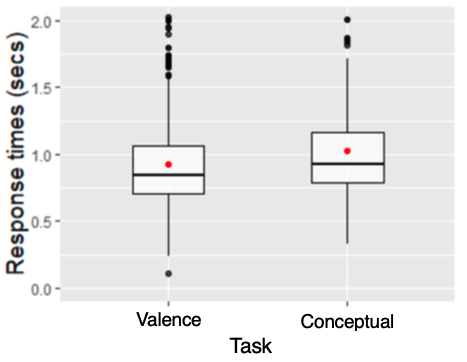
\includegraphics[scale=0.4]{figures/exp1.png}
    \vspace{.2cm}
    \centering
    \captionof{figure}{\small Exp1 Results: Faster RTs for Valence judgments than Conceptual categorization (physical vs. psychological).}
    \label{fig:exp1}
\end{tcolorbox}
\end{minipage}
\hfill
\begin{minipage}{0.48\linewidth}
    \begin{tcolorbox}[colback=white]
    \vspace{-.3cm}
    \centering
    % 
\includegraphics[scale=0.6]{figures/legend.png}
    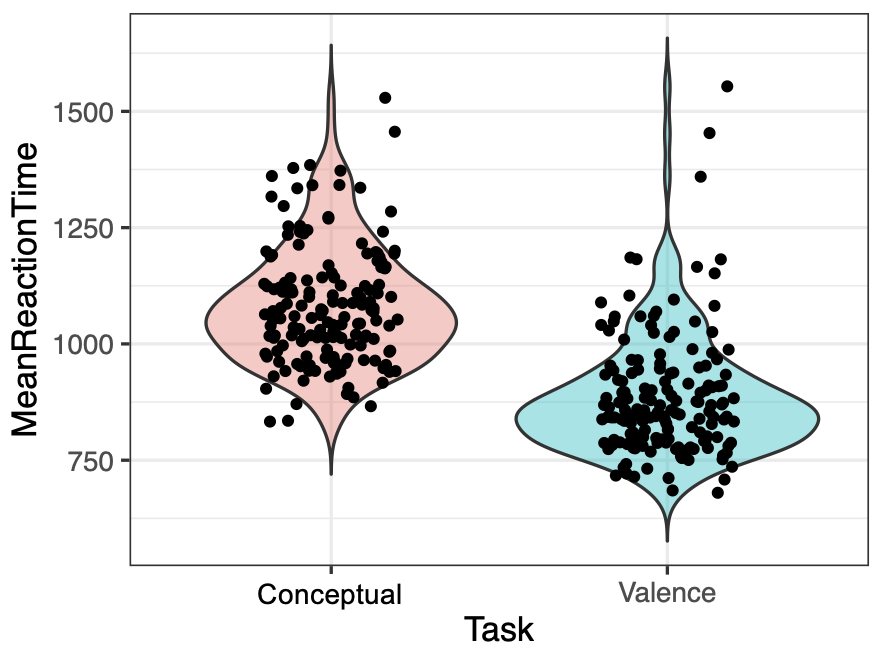
\includegraphics[scale=0.45]{figures/exp3.png}
    \vspace{-.75cm}
    \captionof{figure}{\small Exp2 Results: replication of Exp1 for concrete vs. abstract: $\beta$ = -0.168, $SE$ = 0.0389, $t$ = -4,309, $p$ $<$ .0003}

    \label{fig:exp2}
    \vspace{-.2cm}
    \end{tcolorbox}
\end{minipage}

\vspace{.2cm}

\noindent
\begin{tcolorbox}[colback=white]
\begin{minipage}{0.75\linewidth} 
    \vspace{-.3cm}
    % \hspace{-.5cm}
    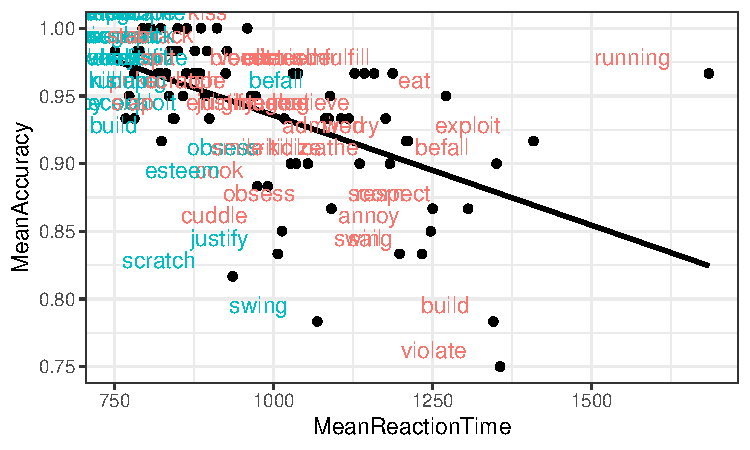
\includegraphics[scale=0.75]{figures/exp1b_accXrt.pdf}
    \vspace{-.2cm}
    % \hspace{1cm}
\end{minipage}
\hspace{-1.5cm}
\begin{minipage}{0.3\linewidth} 
\vspace{-.5cm}
    
\includegraphics[scale=0.5]{figures/legend.png}
    % \vspace{-.7cm}
    % \hrule
    % \vspace{.3cm}
    \captionof{figure}{\small From Exp2, TaskXAccuracy on RT: in Concrete task, responses less accurate and longer ($\beta$ = 0.151, $SE$ = 0.044, $t$ = 3.406, $p$ $<$ 0.0007). However, as accuracy in the Concrete Task increased, reaction time decreased.}
    \label{fig:exp2-items}
    \vspace{-.5cm}
\end{minipage}
\end{tcolorbox}

\begin{tcolorbox}[colback=white]
\begin{minipage}{0.5\linewidth}
    \vspace{-.2cm}
    % \hspace{-.5cm}
    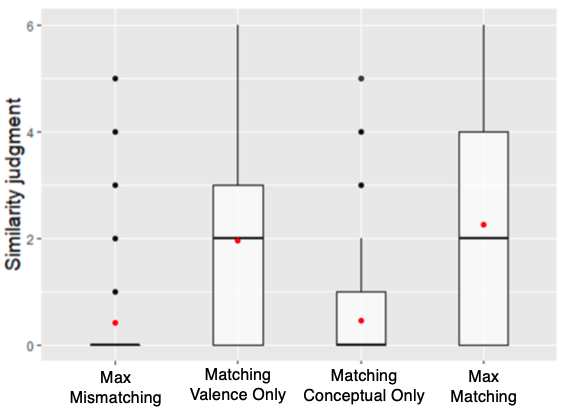
\includegraphics[scale=0.3]{figures/exp2.png}
    \vspace{-.2cm}
\end{minipage}
\begin{minipage}{0.45\linewidth}
    \captionof{figure}{\small Exp3 Results: Similarity judgment task, slider from 0 (dissimilar) to 6 (similar). Participants are more likely to rate verb similarity based on matching Valence (M = 1.97, SD = 1.73), than on matching Conceptual feature (physical/psychological) (M =.47, SD =.88).}
    \label{fig:exp3}
    \vspace{-.5cm}
    % \hspace{1cm}
    
\end{minipage}
\end{tcolorbox}

\small
\noindent \textbf{References}.
[1] Wundt 1907
[2] Zajonc 1980, 2000
[3] Potts 2005 
[4] Schlenker 2007 
[5] Kaplan 1999 
[6] McCready 2010 
[7] Gutzmann 2015 
[8] Stojanovic \& Kaiser 2023 
[9] Stojanovic in press 
[10] Ronderos \& Domaneschi 2023 
[11] Storbeck \& Robinson 2004 
[12] Storbeck \& Clore 2007 
[13] Nummenmaa, Hyönä \& Calvo 2011 
[14] Rohr \& Wentura 2023 
[15] Hinojosa, Moreno \& Ferré 2019 
[16] Hinojosa, Herbert, \& Kissler 2023
[17a] Rohr \& Abdel Rahman 2015 
[17] Levin 1993
[18] Kousta, Vigliocco, Vinson, Andrews and Del Campo 2011 
[18a] Lynott, Connell, Brysbaert, Brand \& Carney 2019 
[19] Vigliocco, Kousta, Della Rosa, Vinson, Tettamanti, Devlin, et al. 2014 
[20] Winter 2022 
[21] Herbert 2023 
[22] Warriner, Kuperman \& Brysbaert 2013,
[23] Brysbaert, Warriner \& Kuperman 2013
[24] Degen 2015 
[25] De Deyne, Perfors and Navarro 2016

\end{document}


